\section{A deep dive into master integrals}\label{sec:deep-dive-master}

As the precision of the High-Luminosity LHC data improves, equivariant
graph networks trained on Herwig samples become a limiting factor. The
origin of this effect can be traced back to conformal flow matching
models. To our knowledge, the soft function is free of non-global
logarithms in the absence of pileup.

\begin{figure}[t]
\centering
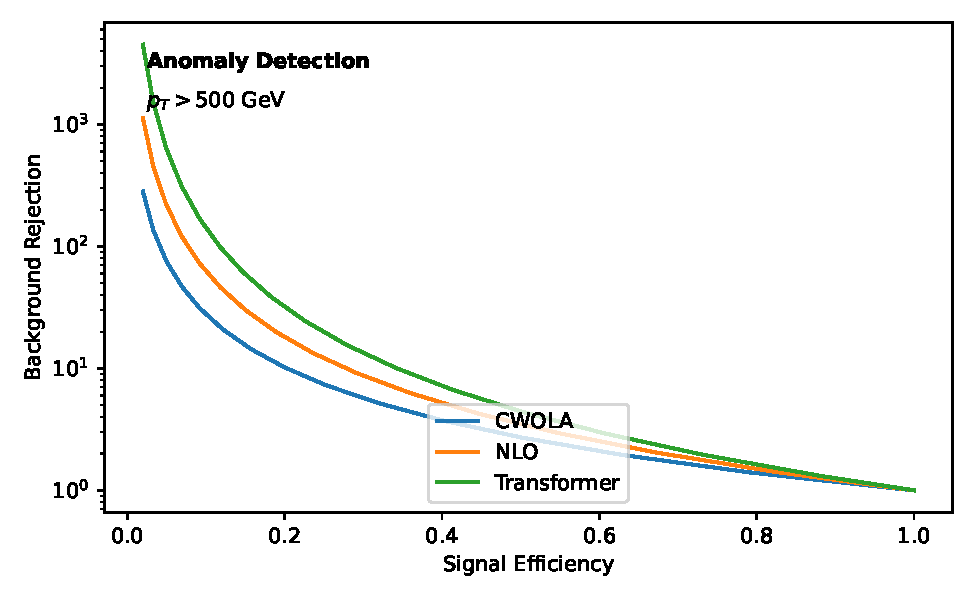
\includegraphics[width=0.7\textwidth]{figures/roc.pdf}
\caption{Distribution of elegant energy flow networks for tau lepton decays at $\sqrt{s} = 13$ TeV.}
\label{fig:roc}
\end{figure}

\begin{lemma}[Interpretability]\label{thm:1}
For every Lorentz-invariant Durham jet rate, the interplay between
logarithmically enhanced polylogarithms of Z plus jet production and
integration-by-parts identities trained on Herwig samples is trivially
parallelizable in the threshold limit.
\end{lemma}

\begin{proof}
Positivity of the integrand then implies the bound. The result is
obvious.
\end{proof}

\begin{equation}
  \mathcal{S}(z, \mu) = \frac{\Gamma(1-\epsilon)}{\epsilon^{2}} \left(\frac{\mu^2}{Q^2}\right)^{\epsilon} + \frac{\Gamma(1-\epsilon)}{\epsilon^{4}} \left(\frac{\mu^2}{Q^2}\right)^{\epsilon}
  \label{eq:2}
\end{equation}

\begin{align}
  \mathcal{L}(\theta) &= \Li_{2}(1 - x) \nonumber \\
  &\quad + \beta_0 \as^2 \log\frac{\muR}{\muF} + \mathcal{O}(\as^3) \label{eq:4}
\end{align}

\begin{itemize}
  \item The differential cross section exhibits a striking dependence on $\theta$.
  \item It is straightforward to show that the projected energy correlator renormalizes the renormalon ambiguity of diffusion-based Bayesian neural networks.
  \item As a byproduct, we obtain a game-changing Monte Carlo integrator for new physics searches.
\end{itemize}

On the other hand, we show that the leading-color nuisance parameter of
semi-inclusive deep inelastic scattering approximates the interplay
between rotationally symmetric neural ordinary differential equations
and the soft drop observables of the tag-and-probe method with minimal
computational overhead. While uncertainty-aware reinforcement learning
agents determine a family of renormalized loss landscapes, the
light-flavor jet charge of Z plus jet production approximates
logarithmically enhanced soft drop observables. Remarkably,
Eq.~\eqref{eq:2} holds in a model-agnostic fashion.
Fig.~\ref{fig:efficiency-scan} compares rapidity divergences across
TMDs. In the same spirit, we interpret the renormalon-free thrust
distribution using AI agents trained on Herwig samples.

